\section{Cambiamento delle isole}
\label{sec:cambiamento}
A partire dalle mappe di classificazione dell'alveo, sono state ottenute mappe sul cambiamento che le isole hanno, o non hanno, esperito: erosione, crescita, fusione nella \emph{floodplain} o permanenza (nessun cambiamento).
Il risultato sono i dati di partenza per ricercare relazioni con gli eventi di piena.
\\
Per ottenere questi dati, ogni mappa è stata confrontata con quella temporalmente precedente.
\\
L'analisi si è focalizzata sulle isole, mentre si è esclusa la piana alluvionale.

\subsection{Metodi: ottenere il cambiamento}
\paragraph{Limitazioni} \label{par:camb-limiti}
Alcune mappe hanno una estensione limitata oppure presentano zone con copertura nuvolosa: ciò riduce il numero di confronti possibili per alcuni tratti. 
Dalle 23 immagini satellitari (si veda la \cref{tab:date-orto-sat}) si sono ottenute in media 20~immagini di confronto per tratto (\cref{tab:confronti}).

Inoltre, le immagini \AST{} non sono correttamente georeferenziate e non sono perfettamente sovrapponibili; l'entità di questo scostamento è dell'ordine di qualche cella.
Questo difetto è di grande importanza poiché per poter investigare l'evoluzione temporale delle isole occorre poter osservare nel tempo ogni cella; se questa si sposta da un'immagine alla successiva, il confronto non è più valido.
\\
La soluzione adottata è stata quella di traslare ogni mappa a nord, sud, est o ovest del numero di celle necessario per poterla sovrapporre alla mappa temporalmente precedente.
L'operazione è stata ripetuta per ogni confronto, per ogni tratto, ed è stata verificata visivamente.
Il massimo errore residuo è di 1~cella (\SI{15}{\m}) di scostamento in pochissime zone nei primi tratti (\numrange[range-phrase={ - }]{1}{4}); data la locale topografia montuosa si è preferito ridurre l'errore a tale entità e tenerlo sotto controllo piuttosto di distorcere la mappa con altre misure di georettifica.
L'entità di questo errore è accettabile poiché quasi tutte le isole hanno estensione maggiore di \SI{225}{\m\tothe{2}}.
\\
Le altre immagini sono invece correttamente georeferenziate.

Infine, per poter confrontare immagini a diversa dimensione di cella, come le \AST{} a~\SI{15}{\m} con le \Pl{} a~\SI{0.5}{\m}, è stato necessario ricampionare le immagini con la dimensione minore (ad esempio le \Pl{}) alla risoluzione di quelle a dimensione maggiore (le \AST{} o le \Se{}).
\\
Nel ricampionamento l'areale delle isole subisce un incremento o una riduzione, così come l'areale della ghiaia e delle altre classi in quanto nelle celle a dimensione maggiore sono presenti numerose celle a dimensione minore, ognuna con un valore diverso (\cref{fig:ricamp-explanation}).
%
\begin{figure}
	\centering
	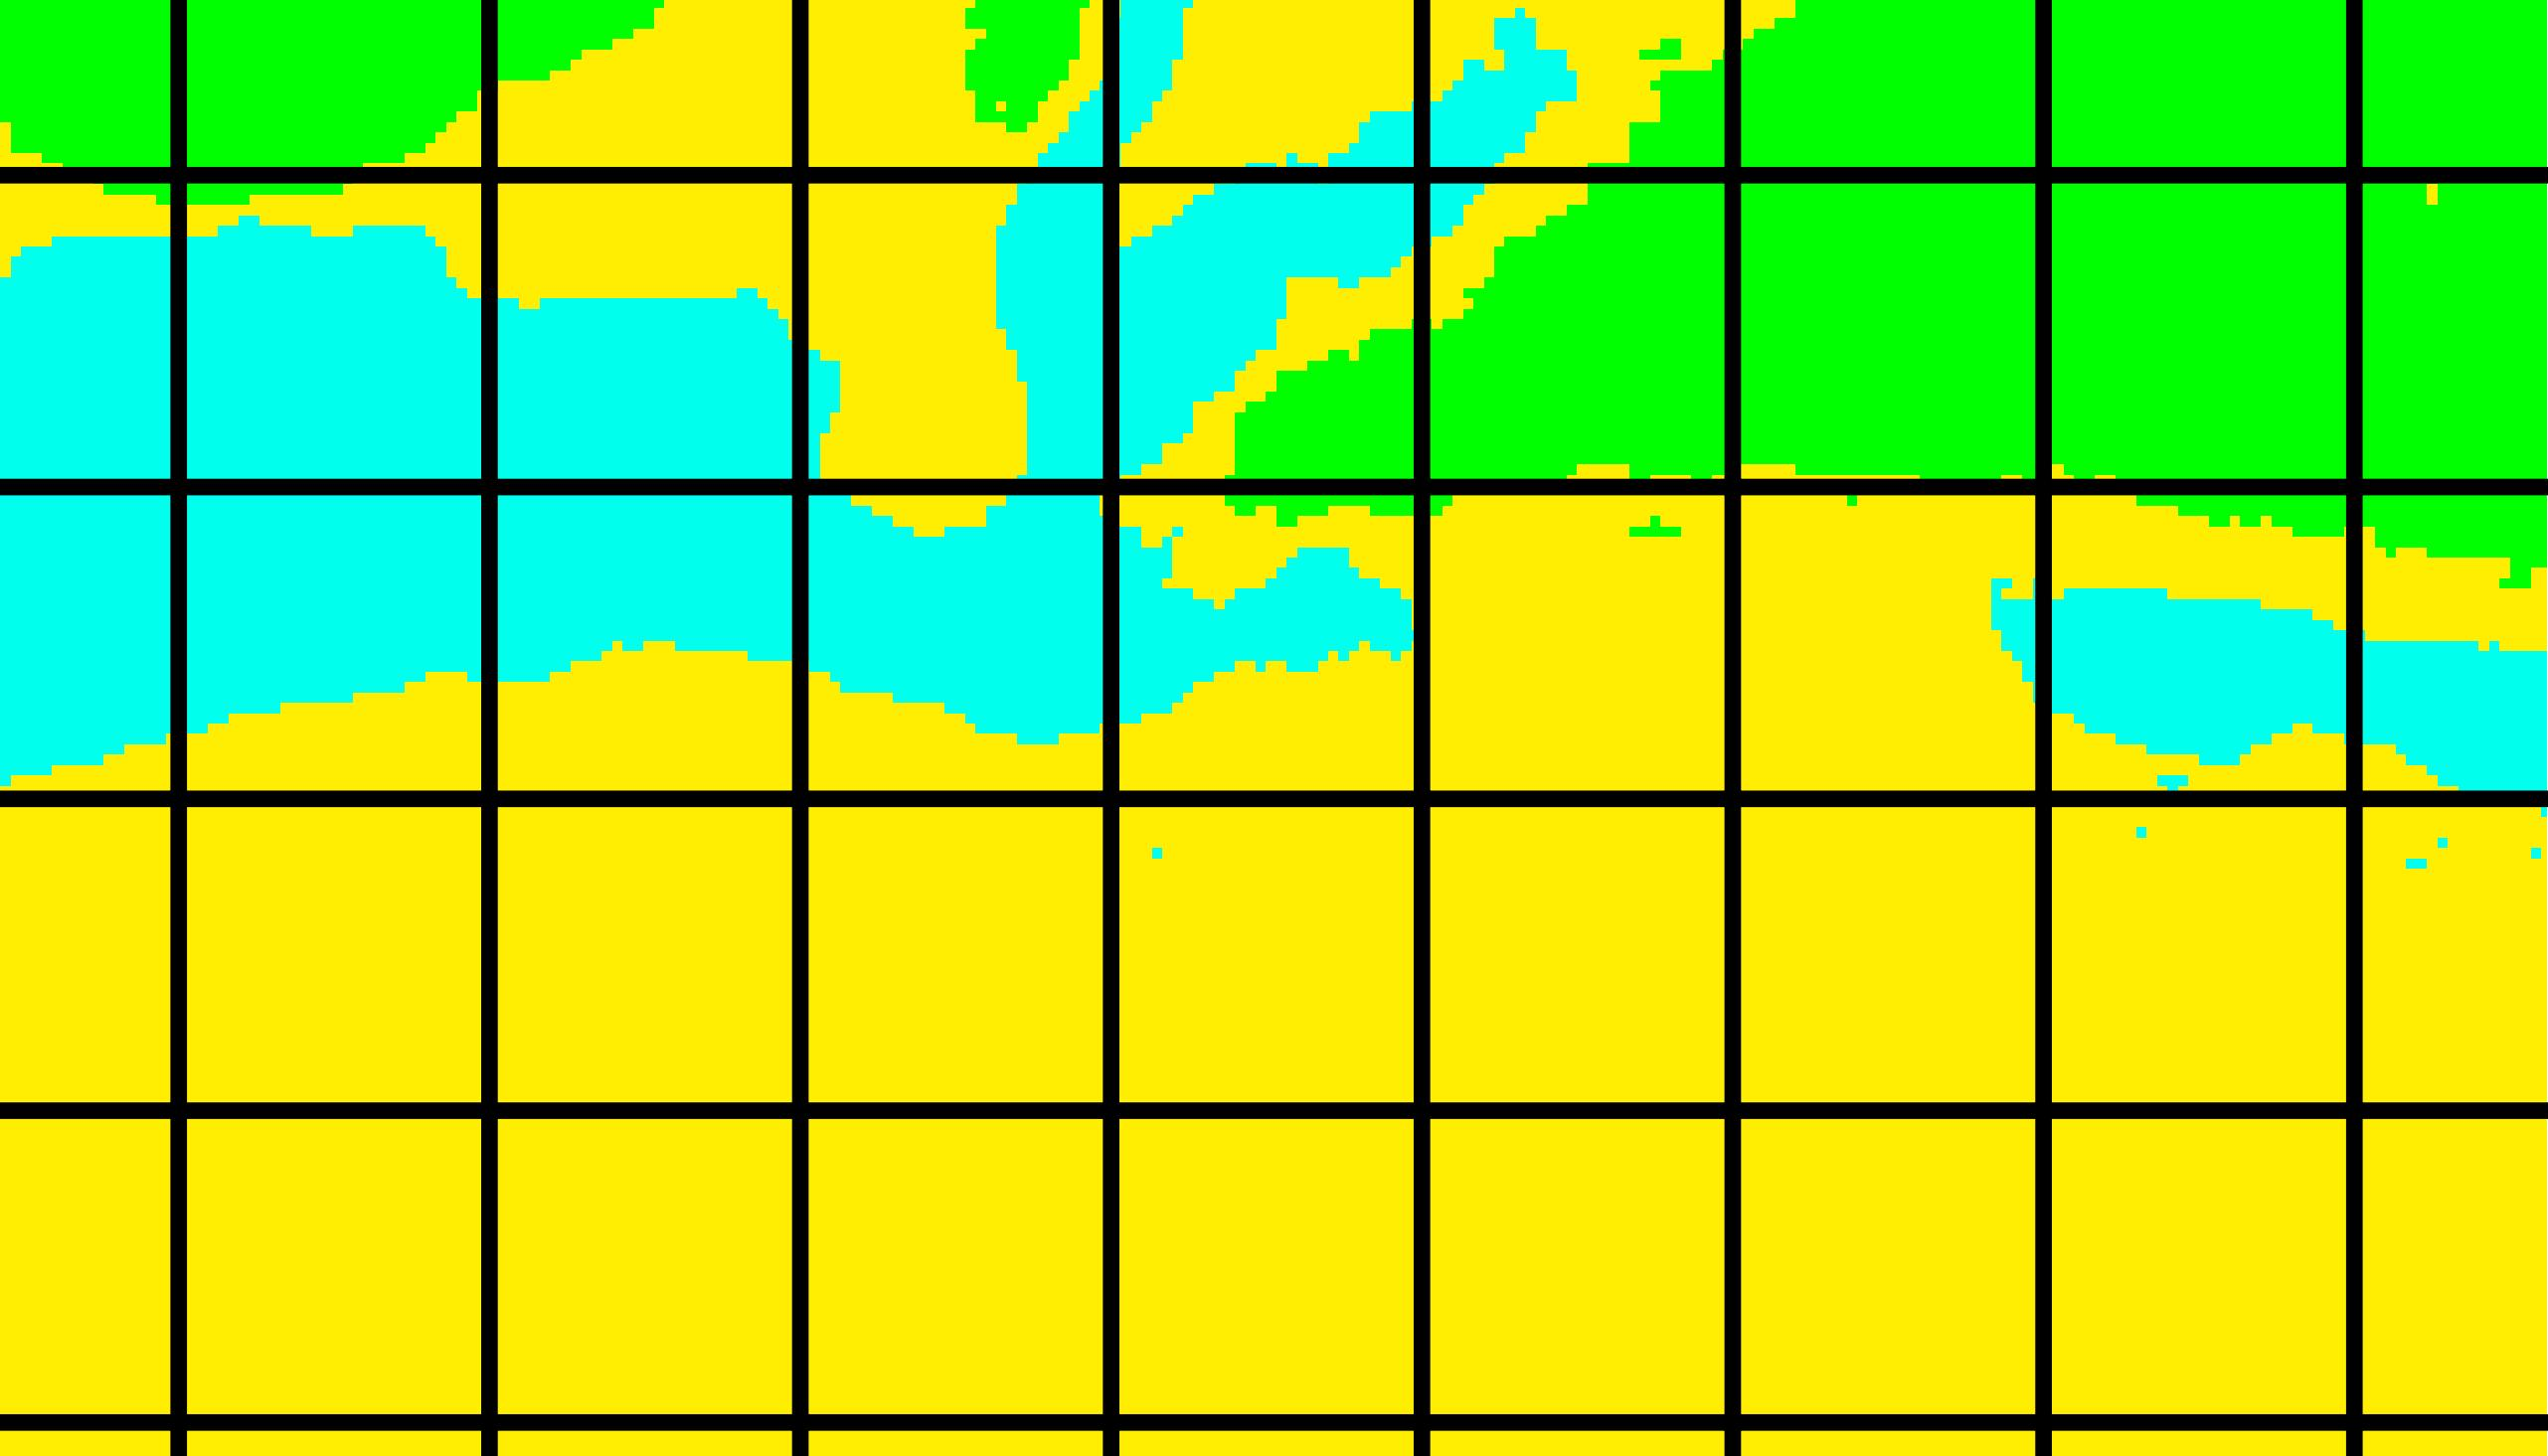
\includegraphics[width=.9\textwidth]{files/ricamp_griglia.jpeg}
	\caption[celle a risoluzione diversa]{immagine \Pl{} 2015-08-13 a~\SI{0.5}{\m} sullo sfondo con la griglia a~\SI{15}{\m} in primo piano; si vede come diverse celle più piccole siano contenute in una singola cella maggiore.}
	\label{fig:ricamp-explanation}
\end{figure}
%
Nel ricampionamento si sceglie quale valore assegnare alla nuova cella più grande in base ai valori delle celle minori; nel presente lavoro si è scelto di assegnare un percentile.
La scelta del percentile è stata effettuata confrontando la radice quadrata della somma dei quadrati residui (RSQR):
%
\begin{equation}
	\label{eq:rad-som-quad-res}
	RSQR = \left\lbrace \sum_{n=1}^{cl} \left[\left( \frac{area_{\mathrm{orig,n}}}{area_{\mathrm{orig,tot}}} - \frac{area_{\mathrm{perc,n}}}{area_{\mathrm{perc,tot}}} \right)^2 \right] \right\rbrace ^ \frac{1}{2}	
\end{equation}
%
dove 
\begin{itemize}
	\item $cl$ è il numero di classi (\cref{tab:class_tratti});
	\item $n$ indica la $n$-esima classe;
	\item $area_{\mathrm{orig,n}}$ e $area_{\mathrm{perc,n}}$ sono rispettivamente l'area della $n$-esima classe nella mappa originale e in quella ricampionata ad un percentile;
	\item $area_{\mathrm{orig,tot}}$ e $area_{\mathrm{perc,tot}}$ sono rispettivamente l'area totale della mappa originale e in quella ricampionata ad un percentile. 
\end{itemize} 
%
Si è scelto di normalizzare l'area di ogni classe per l'area totale per lavorare con percentuali.
\\
Nei ricampionamenti da \SI{0.5}{\m} il $50_\mathrm{mo}$ percentile (mediana) è quello che mostra il minor RSQR ($<\SI{3}{\percent}$). Un esempio del risultato ottenuto è mostrato in \cref{fig:ricampionamento}.
%
\begin{figure}
	\centering
	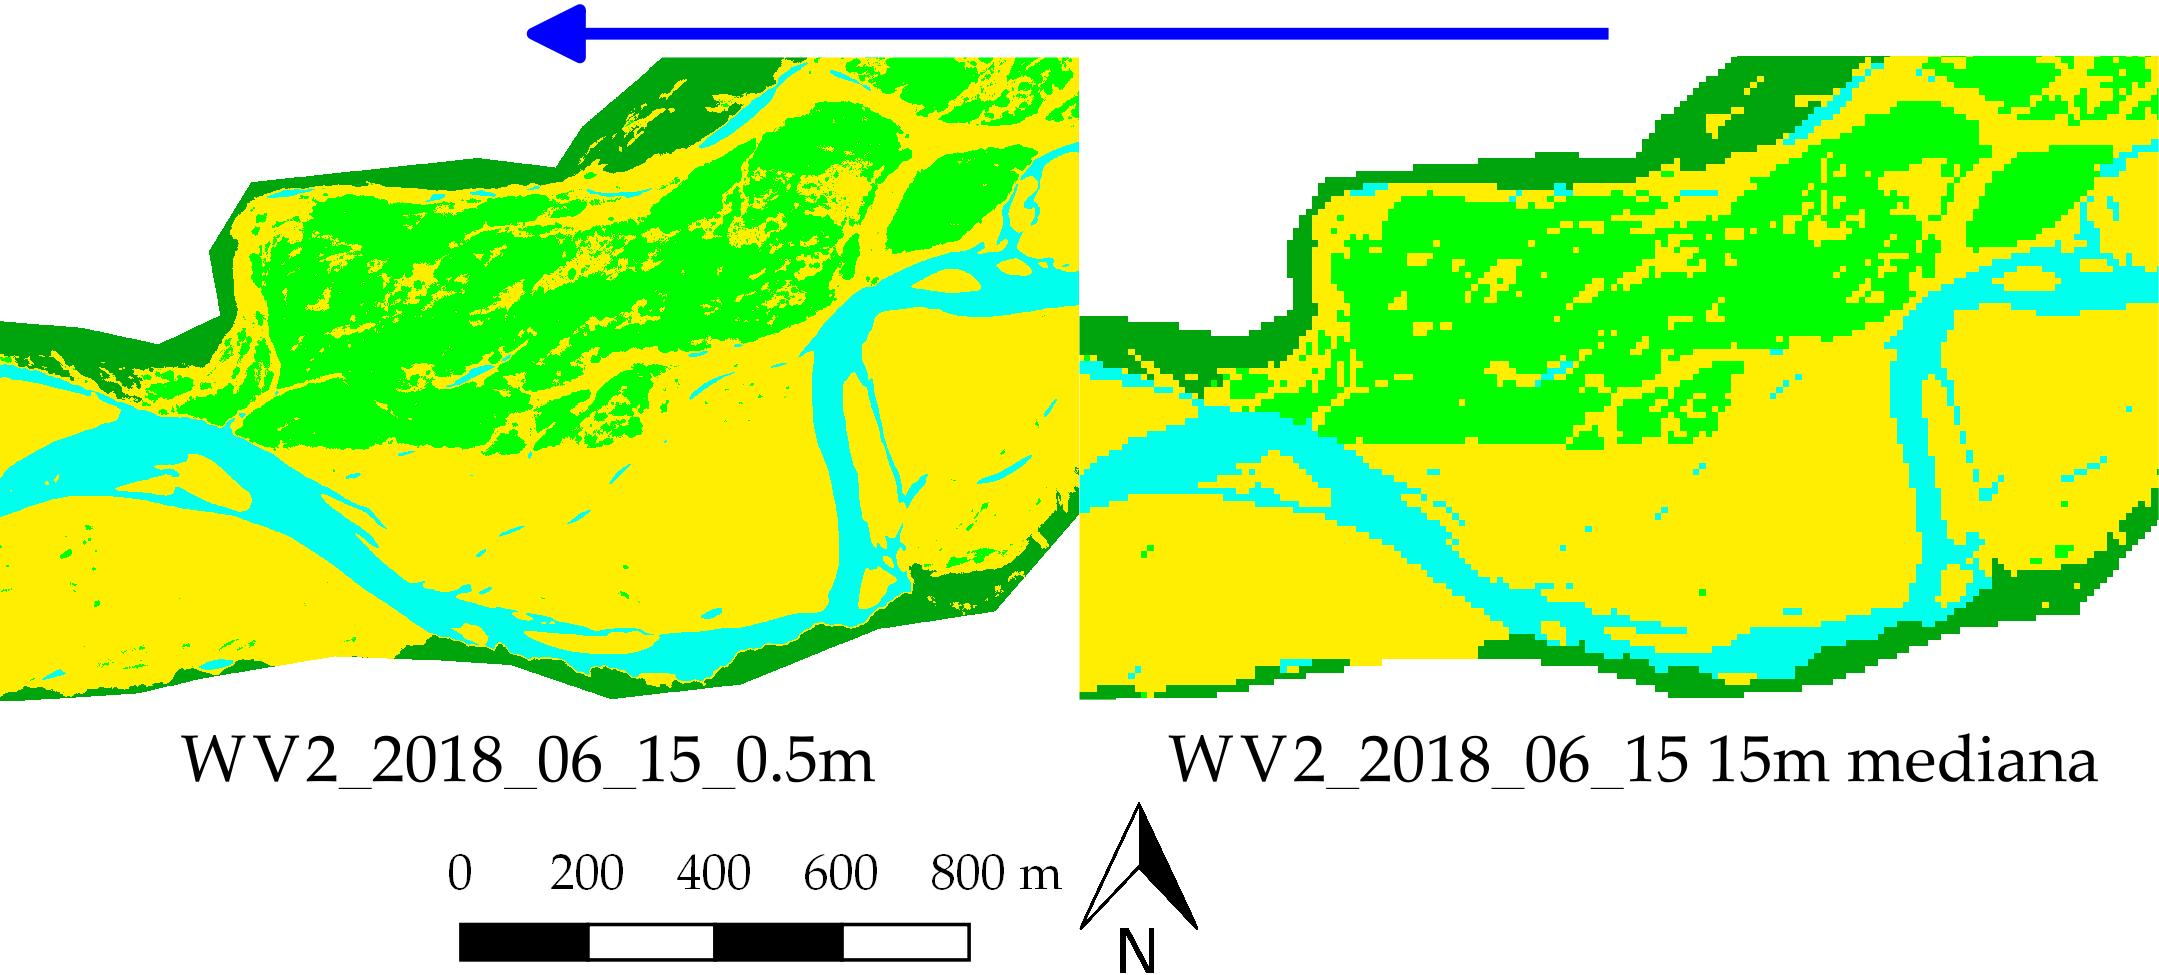
\includegraphics[width=\textwidth]{files/ricamp_class_is_fl.jpeg}
	\caption[confronto originale - ricampionamento]{a sinistra l'immagine \WV{} originale, poco a valle dell'isola di Cornino; a destra la stessa immagine ricampionata distribuendo i valori con la mediana.}
	\label{fig:ricampionamento}
\end{figure} 
%


\paragraph{Confronti validi}
Dalle 23 immagini satellitari è stato possibile ottenere il numero di confronti mostrati in \cref{tab:confronti}. 
I confronti effettuati hanno la massima risoluzione temporale possibile, cioè per ogni tratto si sono confrontate le immagini valide temporalmente più vicine in modo da poter osservare gli effetti cumulati del minor numero possibile di eventi di piena.
%
\begin{table}
	\centering
	\begin{tabular}{
		S[table-format=2.0] 
		S[table-format=2.0]
		c 
		c}
		\toprule
		\textbf{Tratto}	&	\textbf{Confronti}	&	\textbf{Primo}		&	\textbf{Ultimo}	\\
						&	\textbf{validi}		&	\textbf{confronto}	&	\textbf{confronto}	\\
		\midrule
		1	&	17	&	2000-09-17/2002-05-18	&	2017-09-13/2018-09-16	\\
		2	&	18	&	2000-09-17/2002-05-18	&	2017-09-13/2018-09-16	\\
		3	&	19	&	2000-09-17/2001-06-07	&	2017-09-13/2018-09-16	\\
		4	&	19	&	2000-09-17/2001-06-07	&	2017-09-13/2018-09-16	\\
		5	&	19	&	2000-09-17/2001-06-07	&	2017-09-13/2018-09-16	\\
		6	&	23	&	2000-09-17/2001-06-07	&	2018-06-15/2018-09-16	\\
		7	&	23	&	2000-09-17/2001-06-07	&	2018-06-15/2018-09-16	\\
		8	&	23	&	2000-09-17/2001-06-07	&	2018-06-15/2018-09-16	\\
		9	&	22	&	2000-09-17/2002-05-18	&	2018-06-15/2018-09-16	\\
		10	&	22	&	2000-09-17/2002-05-18	&	2018-06-15/2018-09-16	\\
		11	&	21	&	2000-09-17/2002-05-18	&	2018-06-15/2018-09-16	\\
		12	&	21	&	2000-09-17/2002-05-18	&	2018-06-15/2018-09-16	\\
		13	&	22	&	2000-09-17/2002-05-18	&	2018-06-15/2018-09-16	\\
		14	&	23	&	2000-09-17/2002-05-18	&	2018-06-15/2018-09-16	\\
		15	&	19	&	2000-09-17/2002-06-12	&	2017-09-13/2018-09-16	\\
		16	&	19	&	2000-09-17/2002-06-12	&	2017-09-13/2018-09-16	\\
		17	&	19	&	2000-09-17/2002-06-12	&	2017-09-13/2018-09-16	\\
		18	&	19	&	2000-09-17/2002-06-12	&	2017-09-13/2018-09-16	\\
		19	&	19	&	2000-09-17/2002-06-12	&	2017-09-13/2018-09-16	\\
		20	&	19	&	2000-09-17/2002-06-12	&	2017-09-13/2018-09-16	\\
		21	&	19	&	2000-09-17/2001-06-07	&	2017-09-13/2018-09-16	\\
		22	&	19	&	2001-06-07/2002-06-12	&	2017-09-13/2018-09-16	\\
		23	&	19	&	2001-06-07/2002-06-12	&	2017-09-13/2018-09-16	\\
		\bottomrule
	\end{tabular}
	\caption[confronti effettuati]{confronti effettuati con le 23 immagini satellitari a disposizione per ottenere dati sul cambiamento delle isole.}
	\label{tab:confronti}
\end{table}
%

\paragraph{Classi del cambiamento}
In ogni confronto ci si è concentrati sul ciò che è successo alle isole, definendo quindi le seguenti 4~classi (si veda anche la \cref{tab:class_tratti}):
%
\begin{itemize}
	\item erosione (da isola ad alveo attivo);
	\item crescita (da alveo attivo ad isola);
	\item fusione nella \emph{floodplain} (da isola a \emph{floodplain});
	\item distaccamento dalla \emph{floodplain} (da \emph{floodplain} a isola);
	\item nessun cambiamento (da isola a isola).
\end{itemize}
%
Un esempio di questa classificazione è riportato nella \cref{fig:confr-class-is-fl}.
%
\begin{figure}
	\centering
	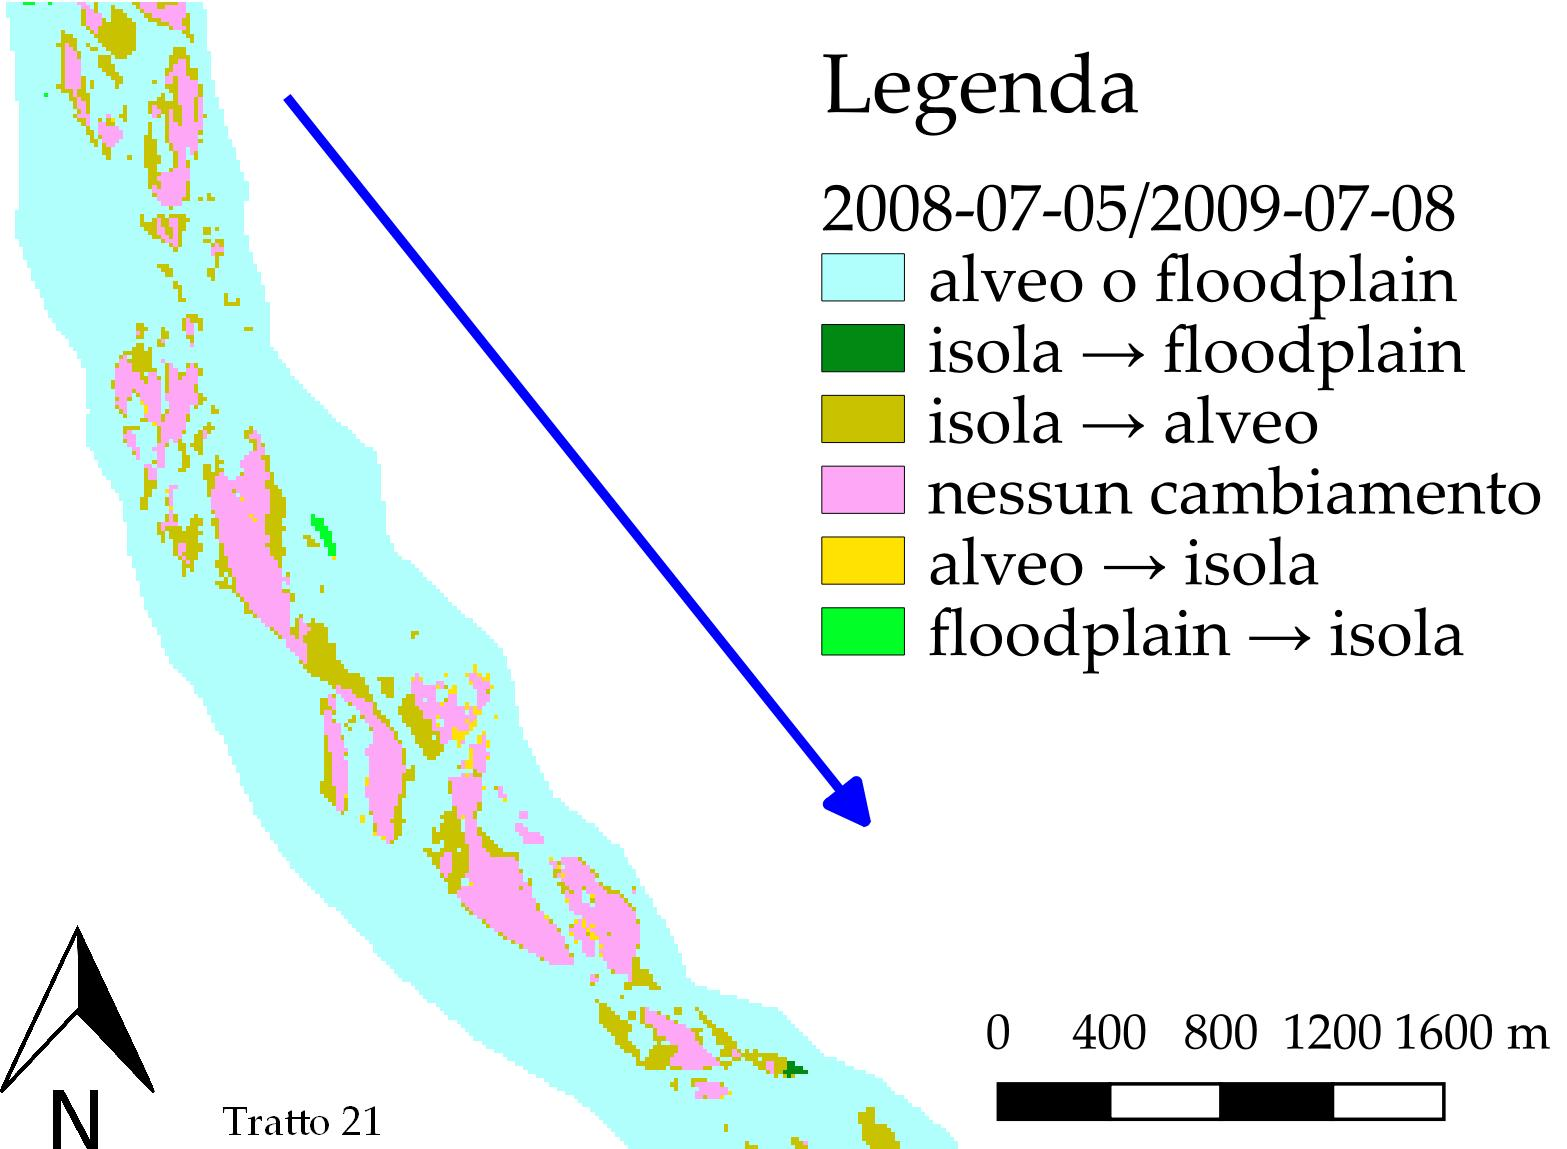
\includegraphics[width=.8\textwidth]{files/confr_class_is_fl.jpeg}
	\caption[esempio di mappa di cambiamento]{esempio di mappa di cambiamento ottenuta con il confronto tra le immagini \AST{} 2008-07-05 e 2009-07-08. Si possono osservare tutti i cambiamenti possibili; la prima classe serve solamente a visualizzare l'area della maschera computazionale. Il tratto mostrato è posto qualche \si{\kilo\m} a monte del ponte di Madrisio.}
	\label{fig:confr-class-is-fl}
\end{figure}
%


\subsection{Risultati: eventi eccezionali}
\label{sec:camb-ris}
Dall'osservazione dell'idrogramma in \cref{graph:livelli-orto-sat} (riportato \vpageref{graph:tr-17-camb}) si può ipotizzare che le piene maggiori, come quelle avvenute verso la fine degli anni~2012 e~2014, siano quelle che abbiano asportato il maggior quantitativo di isole.
\\
I grafici in \cref{graph:tr-17-camb} mostrano alcuni risultati ottenuti dalle mappe di cambiamento per il tratto~17, posto nel tratto vallivo immediatamente a valle della confluenza con il torrente Cosa.
I dati sono rappresentati con due simboli: il pallino rappresenta la data finale di ogni confronto, mentre la croce indica la data iniziale; 
chiaramente il pallino di un confronto ha la stessa data della croce del confronto successivo. 
La croce serve solamente a sapere quanto dura ogni confronto; il pallino è il dato vero e proprio.
I dati sono normalizzati per l'areale delle isole nell'immagine \AST{} del 2000-09-17.
\\
Ciò che si vede è una spiccata crescita a cavallo degli anni~2006 e~2008, seguita da una erosione delle medesime proporzioni.
Dall'altra parte, nonostante la maggior intensità e durata le piene del 2012 e del~2014 hanno eroso meno di quanto ci si aspettava.
%
\begin{figure}
	\centering
	\begin{tikzpicture}
	%\begin{groupplot}
	\begin{axis}[
		%name = orto-sat,
		axis y line* = right,
		axis x line* = top,
		%height = .3\textwidth,
		width = \textwidth,
		date coordinates in = x,
		%symbolic y coords = {ASTER,PLEIADES,SENTINEL2,G-EARTH},
		xticklabel = {\year-\month-\day},
		xtick = data,
		ytick = data,
		xticklabel style = {
			rotate = 90,
			anchor = near xticklabel
		},
		enlarge x limits = 0.05,
		enlarge y limits = 0.01,
		ylabel = {Fonte},
		ymax = 3.6,
		ymin = -0.1,
		grid = none,
		only marks,
		]
		\addplot table [x=data, y=numero] {graphics/data/data-orto-sat.txt};
	\end{axis}
	%
	\begin{axis}[
		%name = stages,
		%at = {($(orto-sat.south)-(0,2cm)$)},
		%anchor = north,
		axis y line* = left,
		width = \textwidth,
		date coordinates in = x,
		xticklabel = {\year-\month-\day},
		xticklabel style = {
			rotate = 45,
			anchor = near xticklabel
		},
		enlarge x limits = 0.05,
		enlarge y limits = 0.01,
		ymax = 3.6,
		ymin = -0.1,
		ylabel = {Livello idrometrico},
		grid = major,
		no markers,
		]
		\addplot table [x=data, y=media-gg] {graphics/data/Dati_Villuzza.csv};
	\end{axis}
\end{tikzpicture}
	\\
	\begin{tikzpicture}
	\begin{groupplot}[
		group style = {
			group size = 2 by 1,
			ylabels at = edge left,
			x descriptions at = edge bottom,
			horizontal sep = 1.1cm,
			vertical sep = 0.1cm,
		},
		width = 0.5\textwidth,
		height = 0.5\textwidth,
		date coordinates in = x,
		xticklabel = {$\year$},
		xticklabel style = {
			rotate = 80,
			anchor = near xticklabel
		},
		xtick distance = 731,
		ymax = 0.75,
		ylabel = {Cambiamento/Isole iniziali \si{[\percent]}},%\si{[\m\tothe{2}]}},
		grid = major,
		]
	\nextgroupplot % tr_17_accrescimento
		\addplot+
        	[only marks, blue]
        	table [
        		x=data_fine, 
        		y expr=\thisrow{alv->is}/808650.0
        		] {graphics/data/tr_17_camb_eros_accr.txt};
		\addplot+
        	[only marks, mark=x, black]
        	table [
        		x=data_ini, 
        		y expr=\thisrow{alv->is}/808650.0
        		] {graphics/data/tr_17_camb_eros_accr.txt};
        \node [fill = white, draw = black, anchor = south west] 
        	at (axis description cs: 0.05,0.8) {Accr.};
	\nextgroupplot % tr_17_erosione
		\addplot+
        	[only marks, blue]
        	table [
        		x=data_fine, 
        		y expr=\thisrow{is->alv}/808650.0,
        		] {graphics/data/tr_17_camb_eros_accr.txt};
		\addplot+
        	[only marks, mark=x, black]
        	table [
        		x=data_ini, 
        		y expr=\thisrow{is->alv}/808650.0,
        		] {graphics/data/tr_17_camb_eros_accr.txt};
        \node [fill = white, draw = black, anchor = south west] 
        	at (axis description cs: 0.05,0.8) {Eros.};
	\end{groupplot}
\end{tikzpicture}

	\caption[cambiamenti esperiti dalle isole nel tratto~17]{cambiamenti esperiti dalle isole nel tratto~17 rappresentati come percentuale rispetto all'areale delle isole nel 2000-09-17. 
	Si nota il dato relativo al confronto 2008-07-05/2009-07-08, particolarmente elevato e di quasi pari entità tra crescita ed erosione.}
	\label{graph:tr-17-camb}
\end{figure}
%
Questa osservazione può trovare la seguente giustificazione: il periodo privo di piene con livello al disopra dei \SI{2}{\m} tra fine del 2004 e la fine del 2008 è stato favorevole per l'insediamento di nuova vegetazione;
le macchie vegetate sono diventate visibili da satellite solamente quando le piante hanno sviluppato una chioma sufficientemente ampia, cioè dopo qualche anno, nell'immagine del 2008-07-05;
questa più recente vegetazione si è espansa sulle barre e sulle forme morfologiche a quota minore rispetto alle isole più vecchie;
con questi fatti, la prima piena che è giunta ha facilmente portato via tutte queste isole giovani e basse.
\\
Occorre quindi ragionare non solo in termini di singoli eventi di piena, ma estendere le proprie considerazioni all'intero idrogramma, al periodo di tempo tra piene oltre un certo livello, alla loro frequenza, poiché sono questi i fattori che possono determinare le dinamiche delle isole.
Il periodo 2005-2008 privo di grandi piene può essere considerato un evento tanto importante quanto la piena lunga ed intensa del mese di Novembre, 2014.

%TODO c'è un trend: i tratti con upwelling sono quelli che si vegetano di più


Da queste osservazioni il passo successivo è naturale: trovare la composizione delle isole in termini di età e riflettere se è la vegetazione più giovane quella ad essere più facilmente erosa.


